\section{Fundamentos}
\label{fundamentos}

En esta secci�n se introducir� algunos conceptos b�sicos que utilizaremos a lo largo del trabajo.


\subsection{Preliminares}

Sea una familia de funciones $\{B_i\}$ en el espacio de funciones continuas en $[a,b]$, se definen

\begin{descripcion1}{Producto interno:}
\begin{align}
\label{def:inner_product}
 \langle B_i, B_j \rangle & \doteq \int_{a}^{b}{B}_{i}(t) \,{B}_{j}(t) \, w(t) dt
\end{align}
\end{descripcion1}

\begin{descripcion1}{Norma:}
\begin{align}
\label{def:norma}
 \| B_i \| & \doteq \sqrt{ \langle B_i, B_i \rangle }
\end{align}
\end{descripcion1}

\begin{descripcion1}{Kronecker delta:}
\begin{align}
\delta_{ij} =
        \left\{
            \begin{array}{ll}
                1 & \mbox{si } i = j \\
                0 & \mbox{si } i \neq j
            \end{array}
        \right.
\end{align}
\end{descripcion1}

\subsubsection*{Ortogonalidad:}
Se dicen que $B_i$ y $B_j$ son ortogonales si se cumple que $\langle B_i, B_j \rangle = 0$

\subsubsection*{Ortogonalizaci�n de Gram-Schmidt:}
Sea $\{v_1, \dots, v_n\}$ una base de un espacio $U$ con producto interno, se define recursivamente
\begin{align}
\label{eq:Gram-Schmidt}
u_i & = \left( v_i - \sum_{i=0}^{i-1}{\langle v_i, u_j\rangle u_j} \right)
\end{align}
Entonces, $\{u_1, \dots, u_n\}$ una base ortogonal y $\left\{\frac{u_1}{\|u_1\|}, \dots, \frac{u_n}{\|u_n\|}\right\}$ es base ortonormal de $U$.


\subsection{Polinomios ortogonales}
Polinomios ortogonales son clases de polinomios $\{B_{i}(t)\}$ definidos sobre el dominio $[a,b]$ que obedecen la relaci�n de ortogonalidad
\begin{align}
\label{eq:ortogonalidad}
\int_{a}^{b}{B}_{i}(t) \,{B}_{j}(t) \, w(t) dt & = 0 \quad\quad \text{cuando $i \neq$} j
\end{align}
donde $w(t)$ es una funci�n peso. Si adem�s cumplen con
\begin{align}
\label{eq:ortonormalidad}
 \int_{a}^{b}{B}_{i}(t) \,{B}_{j}(t) \, w(t) dt & = \delta_{ij}
\end{align}
los polinomios son \textit{\textbf{ortonormales}}. Es decir, est�n normalizados: $ \| B_i \| = 1$


% La tabla \ref{table:polinomios} muestra algunos ejemplos de los polinomios ortogonales: \\
% \begin{table}[!htbp]
% \centering
%     \begin{tabular}{ | l |c |c | c |}
%     \hline
%     \hline
%     \textbf{Polinomio} & dominio & $w(t)$ & $c_{n}$ \\
%     \hline
%     Chebyshev  & $[-1,1]$ & $(1-t^2)$ & $  $ \\[1ex]
%     Legendre   & $[-1,1]$ & $1$       & $ \frac{2}{2\,n+1} $ \\[1ex]
%     Jacobi     & $(-1,1)$ & $(1-t)^{\alpha}\,(1+t)^{\beta}$ & $ $ \\[1ex]
%     \hline
%     \hline
%     \end{tabular}
% \label{table:polinomios}
% \caption{Ejemplos de polinomios ortogonales}
% \end{table}




\subsubsection{Polinomios de Legendre}
\label{legendre}
% Son polinomios ortogonales definidos en $[-1,1]$. Se sabe que el grado de $L_i$ es exactamente $i$,  entonces pueden escribirse como

Si tomamos como funci�n peso $w(t)=1$ en la definici�n \refEQ{def:inner_product} de producto interno, es decir,
\begin{align*}
 \langle L_i, L_j \rangle & = \int_{-1}^{1}{L}_{i}(t) \,{L}_{j}(t)\,w(t)\,dt = \int_{-1}^{1}{L}_{i}(t) \,{L}_{j}(t)\,dt
\end{align*}
se pueden generar los polinomios de Legendre $\{L_i\}$ con el proceso de ortogonalizaci�n de Gram-Schmidt \refEQ{eq:Gram-Schmidt} en el intervalo $[-1,1]$. Normalizando de tal manera que $L_n(1)=1$ da los polinomios de Legendre esperados. Algunos de ellos:
\begin{align*}
L_0(t) &= 1 \\[1ex]
L_1(t) &= t \\
L_2(t) &= \frac{3\,{t}^{2}-1}{2} \\
L_3(t) &= \frac{5\,{t}^{3}-3\,t}{2} \\
L_4(t) &= \frac{35\,{t}^{4}-30\,{t}^{2}+3}{8} \\
 &~ ~\vdots
\end{align*}

% \subsubsection*{Shifted Legendre Polynomials}
Para nuestro prop�sito es conveniente utilizar los polinomios an�logos definido en $[0,1]$, los cuales son llamados \textit{\textbf{shifted} Legendre polynomials},
\begin{align}
\label{eq:legendre}
L_i(t) &= \sum_{j=0}^{i}{ C_{ij}\,t^j }
\end{align}
% donde los coeficientes $C_{ij}$ pueden calcularse con una f�rmula cerrada, ver \cite{abramowitz70a}
el grado de $L_i$ es exactamente $i$.  Se conoce una f�rmula cerrada para el c�lculos de los coeficientes $C_{ij}$ ortonormales. A continuaci�n dicha f�rmula, que puede encontrarse en \cite{abramowitz70a},
\begin{align}
\label{eq:legendre_coefficients}
C_{ij} &= (2\,i+1)^{\frac{1}{2}}\begin{pmatrix}i\cr j\end{pmatrix} {\left( -1\right) }^{j} \begin{pmatrix}j+i\cr j\end{pmatrix}
\end{align}

% \noindent
Pueden verse los primeros diez polinomios de Legendre gr�ficamente en la figura~\ref{fig:legendre}.
\begin{figure}[!htbp]
\vspace*{-0.6cm}
\centering
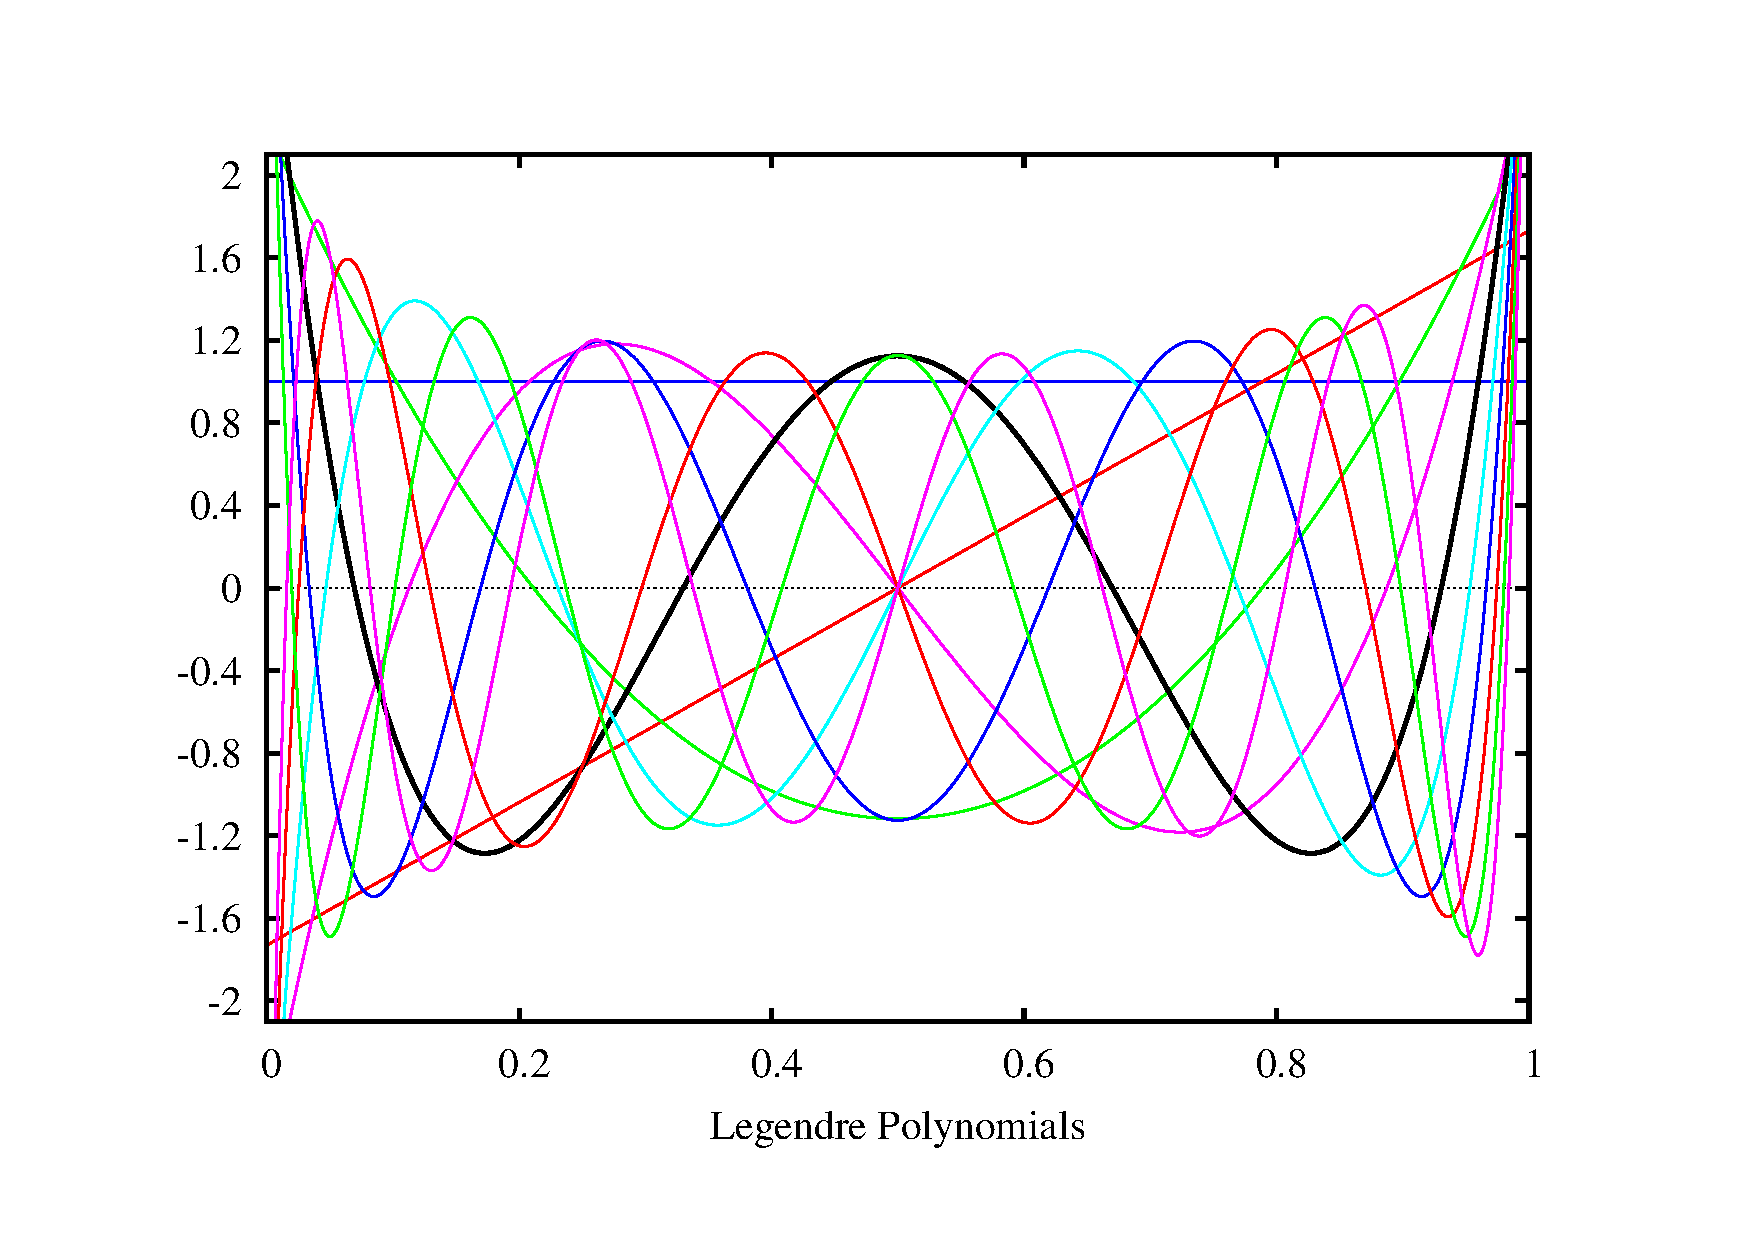
\includegraphics[scale=0.275]{imagen/legendre.pdf}
\vspace*{-0.6cm}
\caption{Primeros diez polinomios de Legendre (shifted) en $[0,1]$}
\label{fig:legendre}
\end{figure}


% \begin{align}
% \begin{split}
% \label{eq:legendre}
% L_i(t) &= \sum_{j=0}^{i}{ C_{ij}\,t^j }\\
% \text{donde} \quad C_{ij} &= (2\,i+1)^{\frac{1}{2}}\begin{pmatrix}i\cr j\end{pmatrix} {\left( -1\right) }^{j} \begin{pmatrix}j+i\cr j\end{pmatrix}
% \end{split}
% \end{align}


\subsubsection{Polinomios de Chebyshev}

(falta)

\subsubsection{Polinomios de Legendre-Sobolev}

(falta)

\subsection{Series de funciones ortogonales}
\label{Series_de_funciones_ortogonales}
\noindent
Si $\{B_i\}$ es una base de polinomios ortonormales respecto al producto interno \refEQ{def:inner_product},
%$L^2[a,b]$,
una funci�n continua~$f$ en el dominio $[a,b]$ puede ser escrita como
\[ f(t) = \sum_{i=0}^{\infty}{\alpha}_{i}\,{B}_{i}(t) \]
Al aplicar el producto interno con $B_i$ en ambos lados de la ecuaci�n anterior se obtiene:
\begin{align*}
\langle f, B_i \rangle & =   \left\langle \sum_{i=0}^{\infty}{\alpha}_{i}\,{B}_{i}(t), B_{i}(t) \right\rangle
                         =   \sum_{i=0}^{\infty} {\alpha}_{i} \langle {B}_{i}, B_i \rangle
                         =   \sum_{i=0}^{\infty} {\alpha}_{i} \delta_{ij}
                         =   {\alpha}_{i}
\end{align*}
Reescribiendo,
\begin{align}
\label{eq:alpha_inner_prod}
{\alpha}_{i} & = \langle f, B_i \rangle
\end{align}
\noindent
Entonces, se puede obtener una aproximaci�n a $f(t)$ al truncar la serie en un cierto orden $d$,
\begin{align}
% \begin{split}
\label{eq:aprox}
f(t) & \approx \sum_{i=0}^{d}{\alpha}_{i}\,{B}_{i}(t)
%      & =  \sum_{i=0}^{d}\langle f, B_i \rangle\,{B}_{i}(t)
\end{align}
